\section{Observations}
\subsection{Attention Sinks Bias Dependency Proxies} \label{obs: attnsinks}

\begin{figure}[t!]
    \centering
    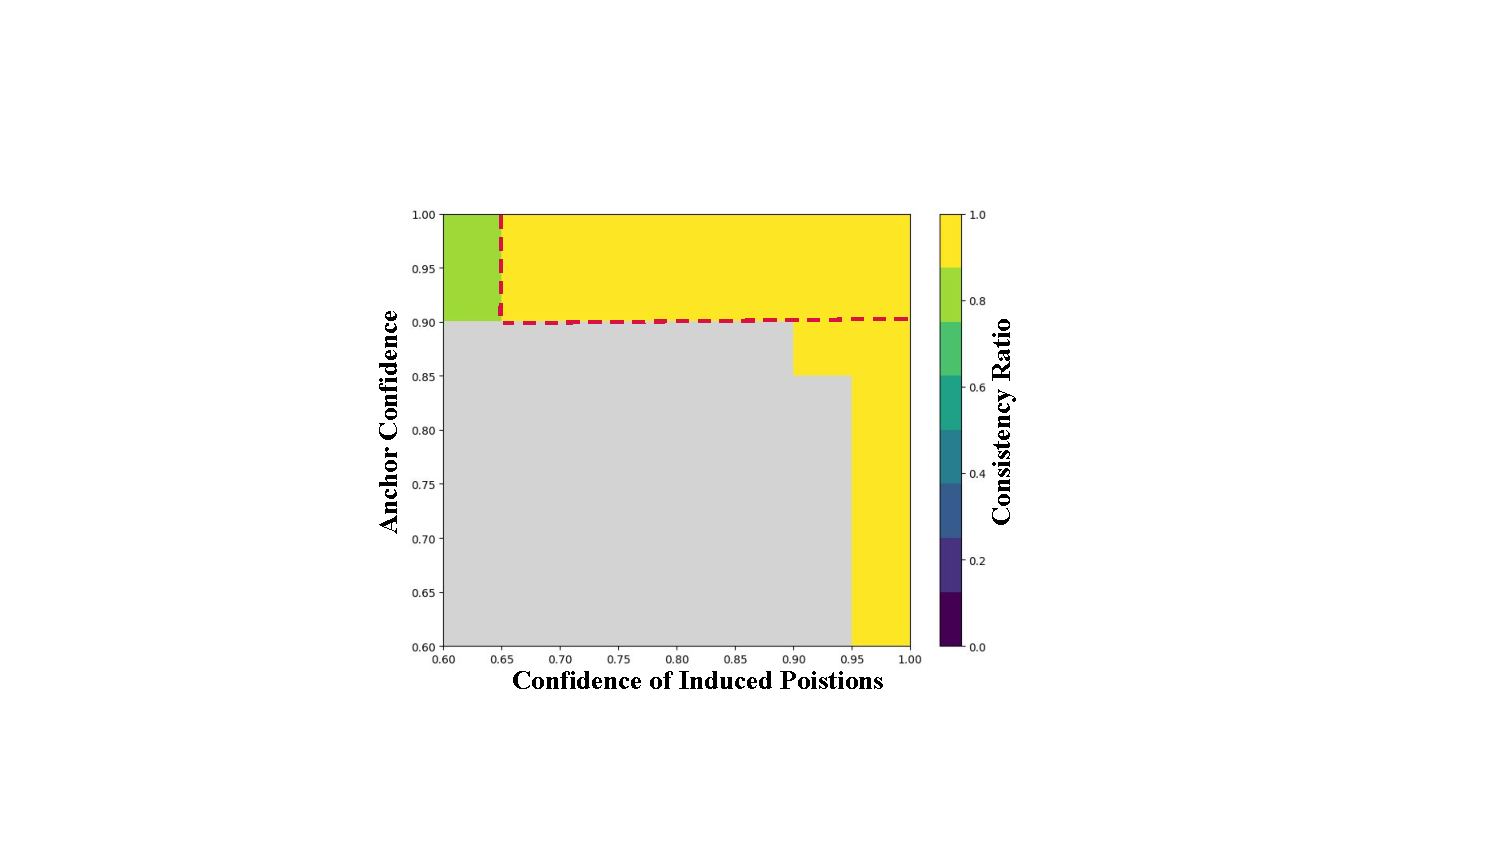
\includegraphics[width=\columnwidth]{fig/anchor.pdf}
    \caption{\textbf{Heatmap of Induced Consistency}  We conduct experiments with LLaDA-8B-Instruct on sampled instances from GSM8K and HumanEval. For each request, we identify coupled pairs where anchors (prompts or previously unmasked tokens) influence induced positions (currently masked positions), and measure whether each induced token’s prediction matches the final decoded output (consistency ratio). Gray cells indicate bins with a negligible fraction of samples and are excluded from analysis.}
    \label{fig:anchor}
\end{figure}

Attention sinks \cite{streamllm, attentionsinksdiffusionlanguage} are common in dLLMs. Across multiple methods and diverse samples, we repeatedly observe an abnormal concentration of attention on a small subset of keys. Moreover, the distribution of concentration is not static. The specific sink tokens and the strength of aggregation can shift as the denoising step progresses. However, this phenomenon appears largely unrelated to the semantics of sink tokens. As shown in Fig.~\ref{fig:attn_sink}, each heatmap exhibits an abnormal concentration of attention mass. Comparing attention maps across denoising steps further indicates that the sink location shifts over iterations. In the rightmost plot, most identified sink tokens are punctuation marks or special tokens with little lexical meaning, suggesting that attention-sink formation is largely independent of token semantics.

\begin{figure*}[t]
    \centering
    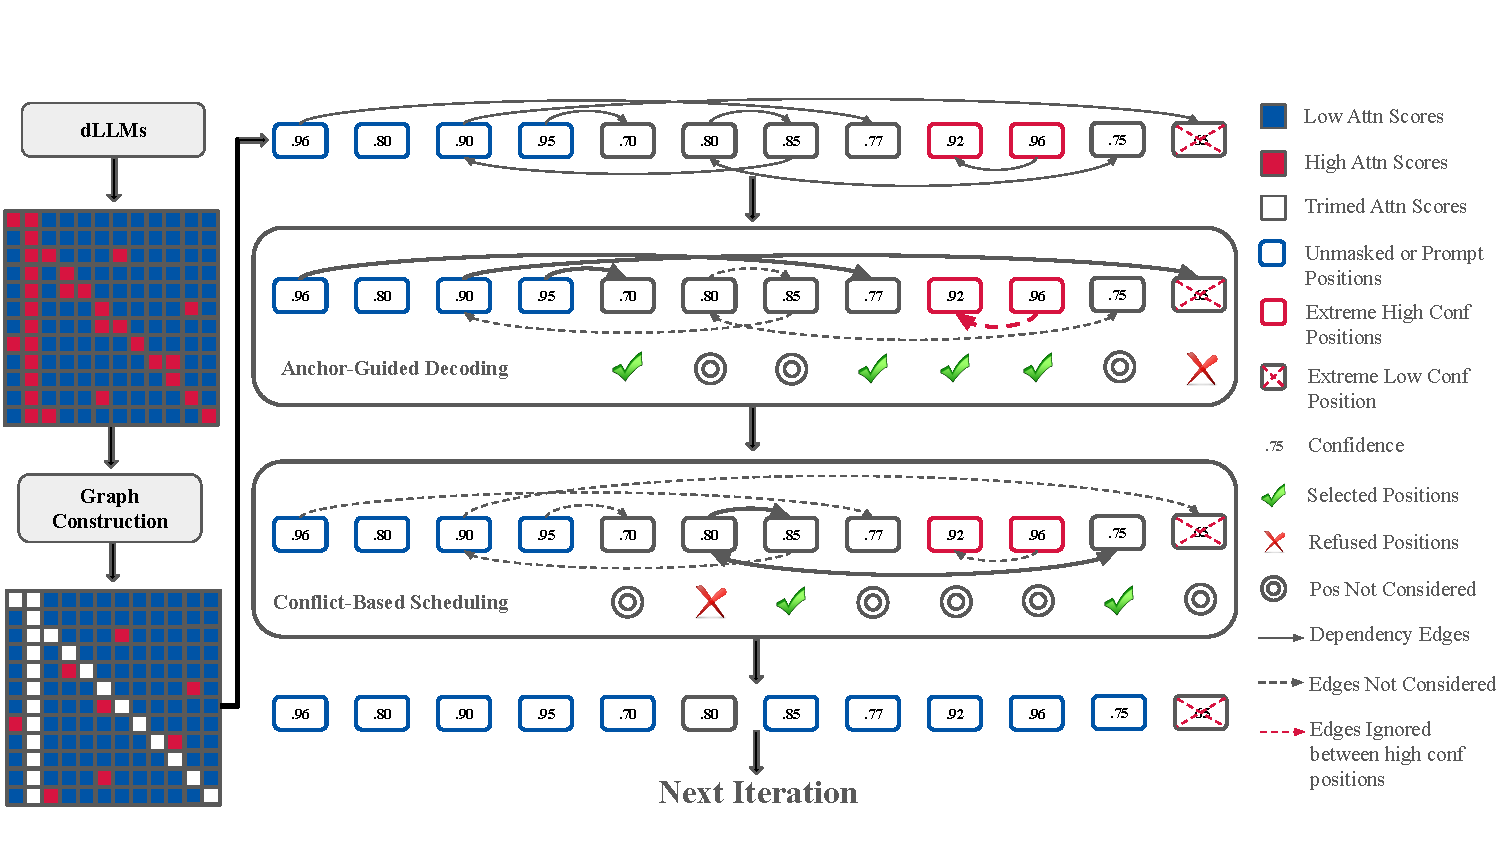
\includegraphics[width=\textwidth]{fig/dawn_arch_1.pdf}
    \caption{\textbf{Overview of \dawn{}.}
    Left: \textit{Dependency Graph Construction} preprocesses the attention map and extracts a sparse directed dependency graph by retaining only salient (high-score) attention links.
    Middle: guided by this graph, \textit{Anchor-Guided Decoding} and \textit{Conflict-Based Scheduling} select two sets of positions, and the union of selected positions is unmasked simultaneously.}
    \label{fig:arch}
\end{figure*}

Attention sinks can be problematic when attention maps are used as a proxy for token dependencies. Sink tokens attract a large amount of attention and can be misinterpreted as exerting strong influence over many other tokens. 
% In fact, this attentional focus does not appear to be driven by semantics.

\subsection{High-Confidence Positions as Anchors} \label{obs: anchors}

During dLLM inference, masked positions can exhibit high consistency even when their confidence is not particularly high. More importantly, we find that the induced positions that are strongly dependent on prompts or previously unmasked tokens with high confidence (anchors) often exhibit high consistency despite relatively low instantaneous confidence. This is validated by the highlighted region in the upper area of Fig.~\ref{fig:anchor}: the induced positions can remain consistent with the final output when their confidence is low. In particular, when the corresponding anchors have confidence above 0.9, the induced tokens are consistently correct at a relatively low confidence. Therefore, the safety of parallel updates depends not only on confidence, but also on whether the prediction is sufficiently conditioned on reliable context. 


